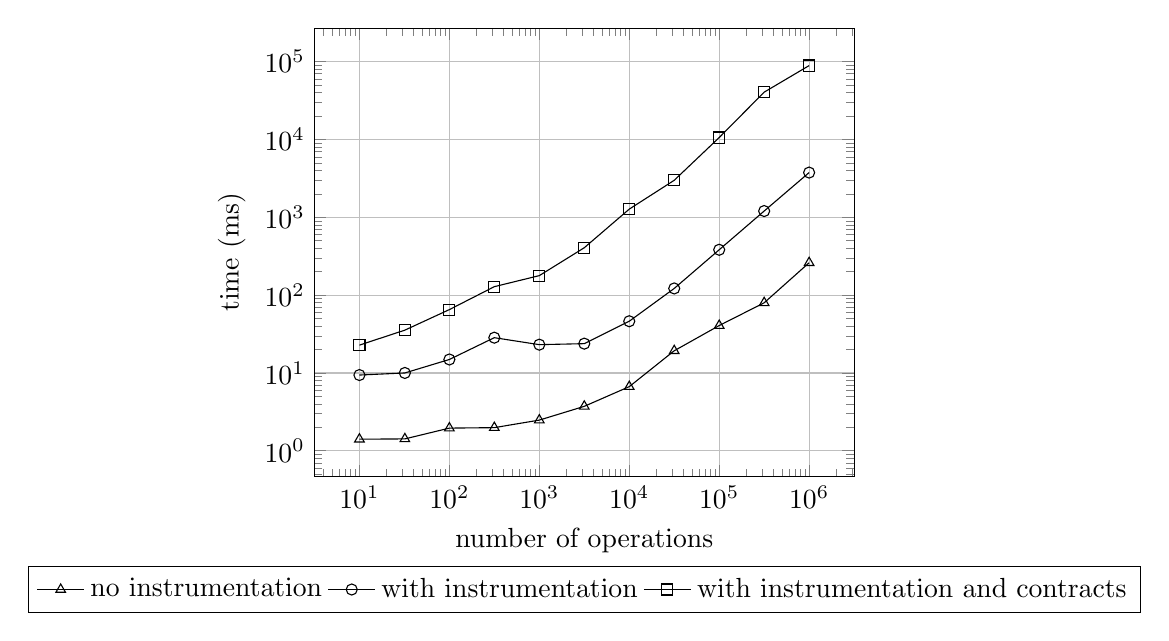
\begin{tikzpicture}
\begin{loglogaxis}[
    xlabel={number of operations},
    ylabel={time (ms)},
    legend style={at={(0.5,-0.2)}, anchor=north,legend columns=-1},
    xmajorgrids=true,
    ymajorgrids=true,
]
\addplot[mark=triangle] coordinates {
    (10,1.40897245) (32,1.420671025) (100,1.95536845) (316,1.982772725)
    (1000,2.47757785) (3162,3.724340825) (10000,6.66815445) (31623,19.277207325)
    (100000,40.665127775) (316227,79.762610275) (1000000,260.9336002)
};
\addplot[mark=o] coordinates {
    (10,9.4) (32,10) (100,14.9) (316,28.4) (1000,23.1) (3162,23.8) (10000,46.2)
    (31623,121.9) (100000,383.1) (316227,1204.7) (1000000,3760.33333333333)
};
\addplot[mark=square] coordinates {
    (10,22.8) (32,35.5) (100,65.2) (316,128.5) (1000,178.2) (3162,406.7)
    (10000,1275) (31623,2992.75) (100000,10600.25) (316227,40595)
    (1000000,89159.6666666667)
};
\legend{no instrumentation, with instrumentation, with instrumentation and
contracts}

\end{loglogaxis}
\end{tikzpicture}
